\chapter{Marco Teórico}

\section{Antecedentes de la investigación}

En el año 2013, Xuan Song, Yayue Pan y Yong Chen de la University of Southern California publican el articulo “Development of a Low-cost Parallel Kinematic Machine for Multidirectional Additive Manufacturing” en el cual ...

\newpage
\section{Bases teóricas}

\subsection{Manufactura}

La manufactura se puede definir de dos maneras \cite{Groover}: una tecnológica y la otra económica. En el sentido tecnológico, la manufactura es la aplicación de procesos físicos y químicos para alterar la geometría, propiedades o apariencia de un material de inicio dado para fabricar piezas o productos; la manufactura también incluye el ensamble de piezas múltiples para fabricar productos. Los procesos para llevar a cabo la manufactura involucran una combinación de máquinas, herramientas, energía y trabajo manual. En el sentido económico, la manufactura es la transformación de los materiales en artículos de valor mayor por medio de uno o más operaciones de procesamiento o ensamblado. La clave es que la manufactura agrega valor al material cambiando su forma o propiedades, o mediante combinar materiales distintos
también alterados. El material se habrá hecho más valioso por medio de las operaciones de manufactura ejecutadas en él.

\subsection{Tipos de Procesos Aditivos}

Los procesos aditivos incluyen, entre otros, todas las tecnologías de prototipado rápido (Rapid Prototyping) con métodos como la impresión 3D: 

\begin{itemize}
    
    \item Inyección de aglutinante (Binder Jetting).
    \item Fabricación con Filamento Fundido (FFF).
    \item Estereolitografía (SLA).
    \item Sinterizado  Láser Selectivo (SLS). 
    \item Polyjet.
    \item Manufactura por Haz de Electrones (EBM).
    \item 3D Bioprinting.
     
\end{itemize}

\subsubsection{Fabricación con Filamento Fundido (FFF)}

La tecnología que ha popularizado la impresión de figuras y piezas en 3D ha sido la que se conoce como fused feposition fodeling (FDM)...

En la figura \ref{fig2} se puede observar una representación esquemática del proceso FFF donde: 

(a) El material plástico es alimentado desde una bobina a un cabezal móvil  (b) que derrite el plástico y lo extruye. El material (c) es depositado capa por capa en la forma deseada sobre una plataforma (e) que baja después de que cada capa es depositada mientras estructuras de soporte auxiliares desechables (d y f) sirven de andamiaje.   
       
% \FloatBarrier sirve para forzar la ubicación de una imagen o tabla. Se coloca antes y despues de la imagen
%\FloatBarrier
\begin{figure}[htbp!]
    % Centrada
    \centering
    % width=0.5 del ancho de hoja y la imagen FDM.png se encuentra dentro de la carpeta gráficos
    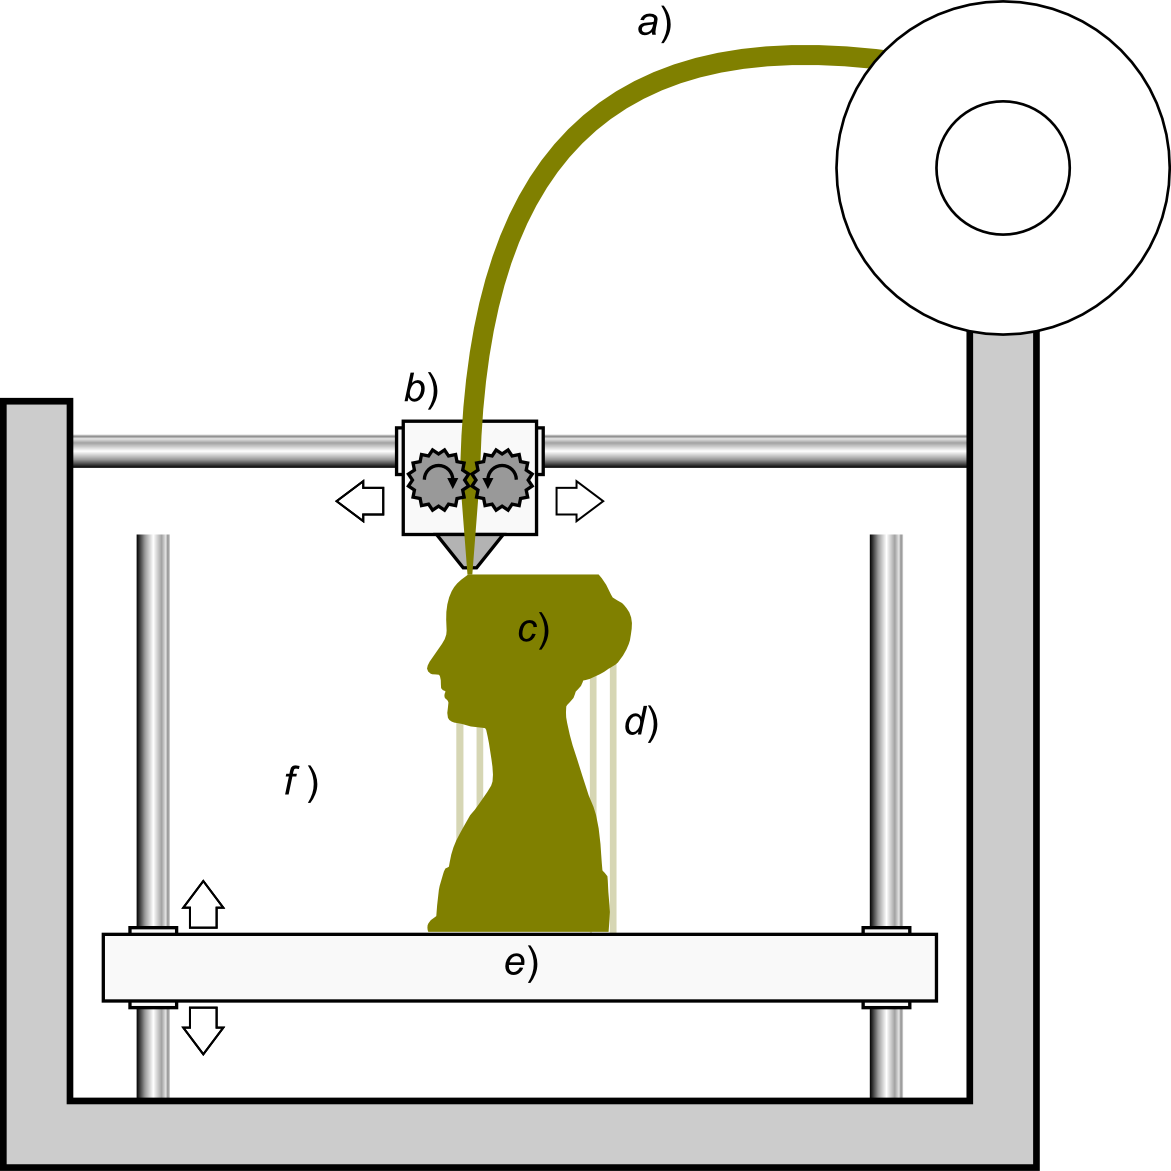
\includegraphics[width=0.5\textwidth]{./graficos/FDM.png}
    % Lo que se muestra debajo
    \caption{Proceso de FFF (Wikipedia).}
    % El alias que le damos para hacer referencia
    \label{fig2}
\end{figure}
%\FloatBarrier

\subsection{Ecuaciones matematicas}

Ecuación centrada y numerada (\ref{eq:ej}):

\begin{equation}\label{eq:ej}
y(x_{i}) = 4 + x_{i}^{2}
\end{equation}

Ecuacion centrada sin numerar 
$$ y(x_{i}) = 4 + x_{i}^{2} $$

Ecuacion en linea $y(x_{i}) = 4 + x_{i}^{2}$, puedes seguir escribiendo.


